\documentclass{beamer}

\usepackage{amsmath,amssymb}
\usepackage{graphicx}
% \usepackage[hidelinks]{hyperref}

\usepackage{setspace}
\doublespacing

\usepackage{subcaption}

\usepackage[sortcites,style=nature,sorting=none,backend=biber]{biblatex}
\addbibresource{ref.bib}

\setbeamertemplate{caption}[numbered]
\renewcommand{\figurename}{Fig.}

\usetheme{Madrid}

\usepackage{minted}  % Core package
\usepackage{xcolor}  % For custom colors
\usepackage{fontspec} % For custom fonts (XeLaTeX/LuaLaTeX only)

% Essential minted configuration for Beamer
\setminted{
    autogobble,
    breaklines,
    fontsize=\footnotesize,
    framesep=2mm,
    obeytabs=true
}

% Fix for Beamer compatibility
\usepackage{catchfile}  % Required for minted in Beamer
\usemintedstyle{friendly}  % Choose a style that works well in presentations

\title[Bacterial Dynamics]{Population Dynamics of Bactria inside Humans}
\subtitle{Battle of Bacteria, Antibiotics and Immune system}
\author[Pooria Mani Naderi]{\small Pooria Assarehha \\ \vspace{-3mm} Mani Moradi \\ \vspace{-3mm} Mohammad Hossein Naderi}
\institute[Dep. Math, Stat \& CS]{Department of Mathematics, Statistics \\ \vspace{-2mm} and Computer Science}
\date{\empty}

\AtBeginSection[]{
  \begin{frame}{Outline}
    \tableofcontents[currentsection]
  \end{frame}
}


\begin{document}
\graphicspath{{../figs/}}

\begin{frame}
    \titlepage
    \vspace{-1.5cm}
    \begin{center}
        
\includegraphics[width=0.18\textwidth]{ut.png}
    \end{center}
    \vspace{-5mm}
    \centering \small Summer 2025
\end{frame}


\section{Introduction}
\begin{frame}
  \begin{itemize}
    \item Bacteria lives inside us
    \item Some of them unwanted
    \item Antibiotics to get rid of them
    \item interactions lead to different equiliberia
  \end{itemize}
\end{frame}

\section{Dynamic Model}

\begin{frame}{Variable Definitions}
  \begin{description}
    \item[$A$]: Concentration of Antibiotics 
    \item[$S$]: Biomass of Non-Antibiotic-Resistant Bacteria 
    \item[$R$]: Biomass of Antibiotic-Resistant Bacteria
    \item[$P$]: Immune Cell Population
    \item[$N$]: $S + R$ total bacteria   
    \item[$\Psi$ and $\Phi$]: functions in \(\mathcal{C}^1(\mathbb{R}_+)\)
  \end{description}
\end{frame}

\begin{frame}{Model Equations}
  Modified Logistic Model
  \begin{eqnarray*} \label{sys}
    \dot{A}(t) & = & \Lambda - \mu A, \\
    \dot{S}(t) & = & \eta_s\left(1 - \frac{S+R}{K}\right)S - \bar{\alpha}AS - \beta\frac{SR}{N} - \Gamma SP, \\
    \dot{R}(t) & = & \eta_r\left(1 - \frac{S+R}{K}\right)R + \beta\frac{SR}{N} - \Gamma RP, \\
    \dot{P}(t) & = & \Phi(N)P\left(1 - \frac{P}{P_{\max}}\right) - \Psi(N)P, \\
  \end{eqnarray*}
\end{frame}

\begin{frame}{Parameter and Term Definitions}
  \begin{description}
    \item[$\Lambda$]: administration rate of Antibiotics
    \item[$\mu$]: absorbtion rate of Antibiotic 
    \item[$\eta_S$ and $\eta_R$]: reproduction rate of $S$ and $R$
    \item[$K$]: carrying capacity (Limiting the reproduction) 
    \item[$\Gamma$]: transfer rate of resistant gene
    \item[$P_{\text{max}}$]: limit of prolifiration of immune cells
  \end{description}
\end{frame}


\begin{frame}{Key Assumptions}
  \begin{columns}
        \column{0.49\textwidth}
  \begin{itemize}
    \item $\eta_S > \eta_R$ cost of resistance
    \item Resistance genes transfer $\beta\frac{SR}{N}$
    \item Immune response $\Gamma S P$ $\Gamma R P$
  \end{itemize}
  \column{0.5\textwidth}
    \begin{figure}
        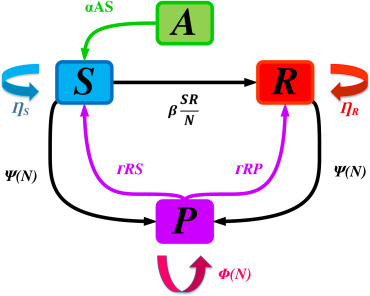
\includegraphics[width=\textwidth]{1-s2.0-S1007570424005975-gr1.jpg}
        \caption{Schematic Diagram}
    \end{figure}
    \end{columns}
\end{frame}


\begin{frame}{Transformation}
\vspace{-20mm}
\[ 
  \begin{array}{ccccc}
    a = \frac{A}{A/\mu} & s = \frac{S}{K} & r = \frac{R}{K} & p = \frac{P}{P_{\max}} & \\
    \alpha = \frac{\bar{\alpha}A}{\mu} & \gamma = \Gamma P_{\max} & n = s + r & \phi(n) = \Phi(Kn) & \psi(n) = \Psi(Kn)
  \end{array}
\]

\vspace{-10mm}

\begin{eqnarray*}
    \dot{a}(t) & = & \mu(1 - a)  \\
    \dot{s}(t) & = & \eta_s(1 - n)s - \alpha as - \beta \frac{sr}{n} - \gamma sp \\
    \dot{r}(t) & = & \eta_r(1 - n)r + \beta \frac{sr}{n} - \gamma rp \\
    \dot{p}(t) & = & \phi(n)p(1 - p) - \psi(n)p 
\end{eqnarray*}

\end{frame}

\begin{frame}{Boundedness}
  \begin{itemize}
    \item \( \mathbb{R}^4_+ = \left\{ (a,s,r,p) \in \mathbb{R}^4 \ | \ a \ge 0 \ s \ge 0 \ , \ r \ge 0 \ , \ p \ge 0  \right\} \)
    \item Right hand side of our system \( \in \mathcal{C}^1 \left(\text{Int}(\mathbb{R}^4_+), \mathbb{R}^4_+\right) \)
    \item Unique Solution exists $\in [0, T_{\max}]$
    \item \(\mathcal{A} = \left\{ (a,s,r,p) \in \text{Int}\left(\mathbb{R}^4_+\right) , a \le 1 , s+r \le 1 , p \le 1 \right\} \) 
    \item lemma: \(\mathcal{A}\) is positively invariant with recpect to \ref{sys} 
    \item hence mathematically and biologically well posed 
  \end{itemize}

\end{frame}

\section{Equiliberia}
\begin{frame}
  Analysing reveals 4 Equilibria - biologically meaningfull
  \begin{itemize}
    \item clearance of infection
    \item infection under $S$
    \item infection under $R$
    \item infection under both
  \end{itemize}
\end{frame}

\begin{frame}[shrink=20]{deriving Equilibria}
  \begin{columns}
    \column{0.65\textwidth}
      \begin{itemize}
          \item Equiliberia $\equiv$ Zero Change $\equiv$  \( \dot{\mathbf{X}} = \vec{0} \)
          \item let \(f(n) = 1 - \frac{\psi(n)}{\phi(n)}\) with \(f(0)>0\) and simplify
          \item we want \( f \uparrow \) for small \(n\) and \(f \downarrow \) for large \(n\) (How Immunity works)
          \item \(f\) either remains \(+\) or after a threshold drops \(< 0\)
          \item we focus on 2nd scenario (remmeber \( n \) is bounded )
      \end{itemize}
    \column{0.34\textwidth}
      \begin{figure}
        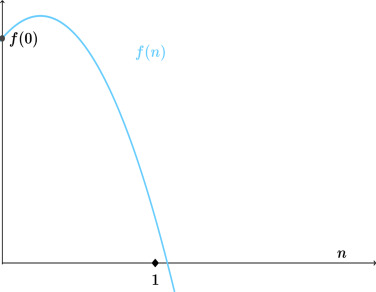
\includegraphics[width=\textwidth]{1-s2.0-S1007570424005975-gr2.jpg}
        \caption{Schematic Rep. of what \(f\) can be}
      \end{figure}
  \end{columns}
  \vspace{-5mm}
  \[\begin{array}{l}
    \mu(1 - a)  = 0 \\
    \eta_s(1 - n)s - \alpha as - \beta \frac{sr}{n} - \gamma sp = 0 \\
    \eta_r(1 - n)r + \beta \frac{sr}{n} - \gamma rp = 0 \\
    \phi(n)p(f(n) -p ) = 0 
  \end{array} \quad \Rightarrow \quad \begin{array}{l}
    a = 1 \\
    s = 0 \quad \text{or} \quad \eta_s(1-n) - \alpha - \beta\frac{r}{n} -\gamma p =0 \\
    r = 0 \quad \text{or} \quad \eta_r(1-n) + \beta\frac{s}{n} -\gamma p =0 \\
    p = 0 \quad \text{or} \quad p = f(n) \\
  \end{array} \]
\end{frame}

\begin{frame}{Equiliberia}
  7 Cases 
\begin{itemize}
  \item Case 1: \(E_0 (1,0,0,0) \)   \(r = s = p = 0\)
  \item Case 2: \(E_1 (1,0,0,f(0)) \)   \( r = s = 0 \ , \ p \neq 0 \)
  \item Case 3: \(E_2 (1,0,1,0) \)   \( s = p = 0 \ , \ r \neq 0 \)
\end{itemize}
\end{frame}

\begin{frame}[shrink= 10]
  \frametitle{Case 4}
  Case 4: \(E_+ \)  \( s = 0 \ , \ r \neq 0 \ , \ p \neq 0 \) 
  \[ r = \lambda_+ \quad p = f(\lambda_+) \quad \Rightarrow f(r) = \eta_r \frac{1 - r}{\gamma} \]
  \vspace{-10mm}    
  \begin{figure}
      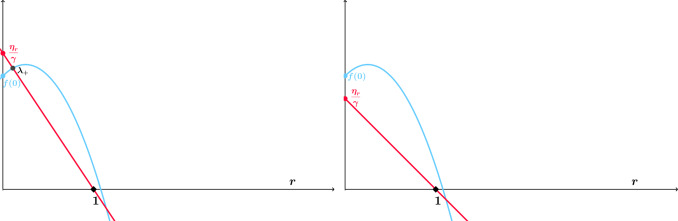
\includegraphics[width=0.7\textwidth]{1-s2.0-S1007570424005975-gr3.jpg}
      \caption{\(f\) and \(\lambda_+\)}
  \end{figure}
  \vspace{-5mm}
  if \( f(0)  < \frac{\eta_r}{\gamma} \) exists Unique \( 0 < \lambda_+ < 1 \)  
\end{frame}

\begin{frame}[shrink= 20]{Case 5 an 6 }
  \begin{itemize}
    \item Case 5 \(E_3(1,1-\frac{\alpha}{\eta_s},0,0)\)
   \(s \neq 0 \ , \ r = 0 \ , \ p = 0 \) 
    \item Case 6 \( E_- \) 
    \(s \neq 0 \ , \ r = 0 \ , \ p \neq 0 \) 
    \[ s = \lambda_- \quad , \quad p = f(\lambda_-) \Rightarrow f(s) = \frac{\eta_s- \alpha}{\gamma} - \frac{\eta_s}{\gamma}s\]
    
     \begin{figure}
    	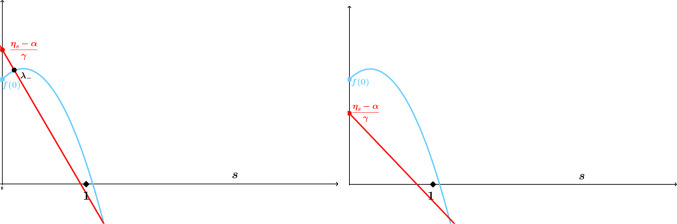
\includegraphics[width=0.7\textwidth]{1-s2.0-S1007570424005975-gr4.jpg}
    	\caption{\(f\) and \(\lambda_-\)}
    \end{figure}
    
    Like Case 4 if \( f(0) < \frac{\eta_s- \alpha}{\gamma} \) exists Unique \( 0  < \lambda_- < 1 \) 
  \end{itemize}

\end{frame}

\begin{frame}{Case 7: \(E_*\) }
    \(s \neq 0 \ , \ r \neq 0 \ , \ p \neq 0 \)

    \(n_* = s + r = 1 - \frac{\alpha + \beta}{\eta_s - \eta_r}\)

    \(n_* > 0 \) if \(\alpha + \beta + \eta_r < \eta_s \)
    \[ \begin{array}{l}
       p_* = f(n_*) \\
       s_* = \frac{n_*}{\beta}\left( \gamma f(n_*) - \eta_r \frac{\alpha + \beta}{\eta_s - \eta_r} \right) \\
       r_* = \frac{n_*}{\beta}\left( \eta_s \frac{\alpha + \beta}{\eta_s - \eta_r} - \alpha - \gamma f(n_*) \right)
    \end{array} \]    
    \[ p_* \ , \  s_* \ , \  r_* > 0 \qquad  \text{if} \qquad \eta_r \frac{\alpha + \beta}{\eta_s - \eta_r} < \gamma f(n_*) < \frac{\alpha \eta_r + \beta \eta_s}{\eta_s - \eta_r} \]  
\end{frame}

\section{Stability Analysis}
\begin{frame}[shrink = 25]{Linearinzation}
    \begin{itemize}
      \item System is non linear,
      \item Linearinzation around fixed points \(\Rightarrow\) Jacobian Matrix
      \item Signs of the eigenvalues of the Jacobian matrix shall be determined
\[
\begin{pmatrix}
-\mu & 0 & 0 & 0 \\
-\alpha s & \eta_s (1-n) - \eta_s s - \alpha a - \beta \frac{r^2}{n^2} - \gamma p & -\eta_s s - \beta \frac{s^2}{n^2} & -\gamma s \\
0 & -\eta_r r + \beta \frac{r^2}{n^2} & \eta_r (1-n) - \eta_r r + \beta \frac{s^2}{n^2} - \gamma p & -\gamma r \\
0 & \phi(n) (f(n)-p) + \dot{f}(n) p \phi(n) & p \dot{\phi}(n) (f(n)-p) + \dot{f}(n) p \phi(n) & \phi(n) (f(n)-2p)
\end{pmatrix}
\]

     \item let  \(
C_{+} = \eta_{s}\left(1 - \lambda_{+}\right) - \alpha - \beta\), \( C_{-} = \eta_{r}\left(1 - \lambda_{-}\right) + \beta\)
and 
\vspace{-0.2cm} % Adjust spacing
\[
C_* = -\frac{\left(\eta_s s_* + \eta_r r_*\right) \beta s_* r_* \left(\eta_s - \eta_r\right)}{f(n_*)\phi(n_*) (n_*)^2 \left(\eta_s s_* + \eta_r r_* + f(n_*)\phi(n_*)\right)} - \frac{\eta_s s_* - \eta_r r_*}{\eta_*} .
\]
will show up for finding stability criteria 
    \end{itemize}

\end{frame}

\begin{frame}[shrink = 25]{Stability Table}
  \begin{table}[ht]
\centering
\caption{Conditions for the stability of equilibria.}
\label{tab:stability}
\begin{tabular}{l|l|l}
\hline
\textbf{Equilibrium} & \textbf{Biological existence} & \textbf{Stability} \\
\hline
\hline
\( E_0 \ (1, 0, 0, 0) \) & Always exists & Always unstable \\ 
\( E_1 \ (1, 0, 0, f(0)) \) & Always exists & \(\alpha > \eta_s\) and \(\gamma f(0) > \eta_r\) \\
\( E_2 \ (1, 0, 1, 0) \) & Always exists & Always unstable \\
\( E_3 \left(1, 1 - \frac{\alpha}{\eta_s}, 0, 0\right) \) & \(\eta_s > \alpha\) & Always unstable \\
\( E_+ \ (1, 0, \lambda_+, f(\lambda_+) ) \) & \(\eta_r > \gamma f(0)\) & \(\gamma f(\lambda_+) > C_+\) and \(\gamma f(\lambda_+) > \eta_r\) \\
\( E_- \ (1, \lambda_-, 0, f(\lambda_-)) \) & \(\eta_s - \alpha > \gamma f(0)\) & \(\gamma f(\lambda_-) > C_-\) and \(\gamma f(\lambda_-) > \eta_s\) \\
\( E_* \ (1, s_*, r_*, f(n_*) ) \) & 
\(\begin{cases}
\eta_r \frac{\alpha + \beta}{\eta_s - \eta_r} < \gamma f(n_*) < \frac{\eta_r \alpha + \eta_s \beta}{\eta_s - \eta_r} \\
\text{and} \\
\eta_s > \eta_r + \alpha + \beta
\end{cases}\) & 
\(\gamma f(n_*) > C_*\) \\
\hline
\hline
\end{tabular}
\end{table}
\end{frame}

\section{Numerical Computation}
\begin{frame}[shrink= 25]{Numerical Computation}
\begin{itemize}
	\item we have chosen the function $f(n)=-n^2+n+\frac{3}{4}$ the aligns with our hypothesis
	 \vspace{1mm}  
	\begin{figure}
			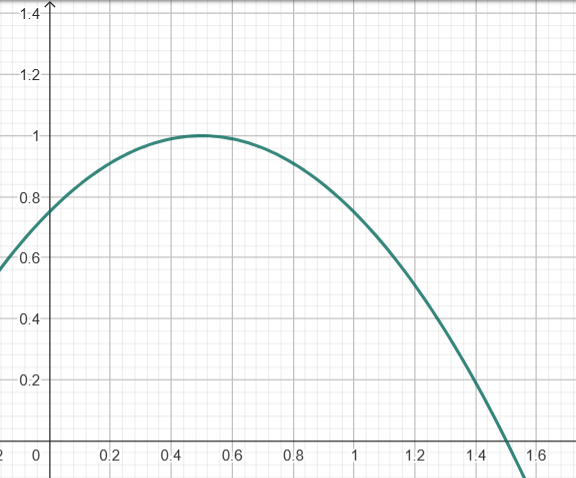
\includegraphics[width=0.3\textwidth]{Screenshot 2025-08-04 174654.png}
		\caption{$f(n)=-n^2+n+\frac{3}{4}$}
	\end{figure}
	\item Since $E_1$ is the equilibria which the system will reach an infection free state we will display it
\end{itemize}

\end{frame}

\begin{frame}{Numerical Computation}
\begin{figure}
		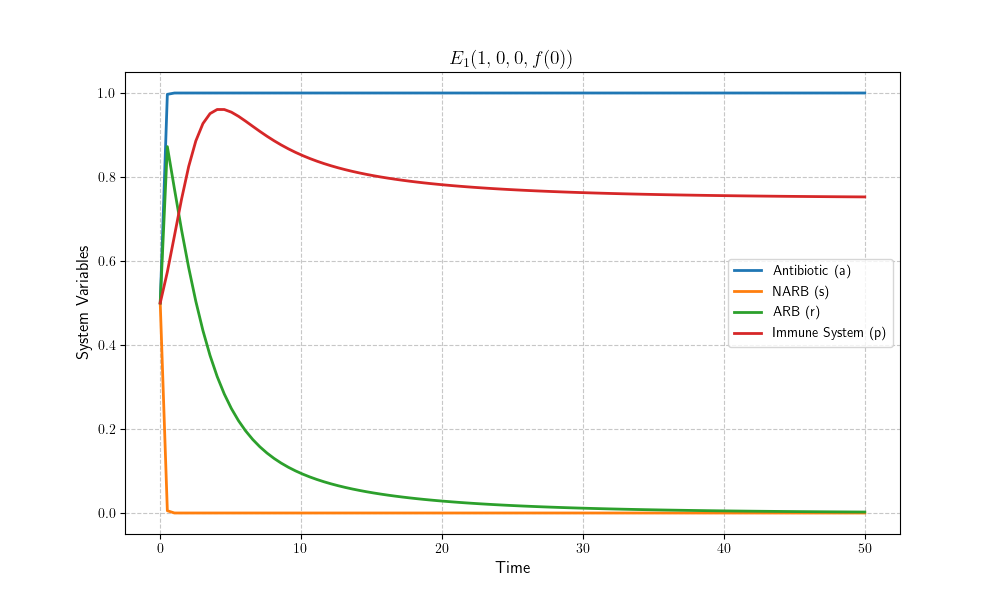
\includegraphics[width=0.9\textwidth]{equiliberia1.png}
        \caption{Stability of $E_1$}
\end{figure}	

\end{frame}

\begin{frame}{Numerical Computation}
	
	Specifically, for $E_1$ to be stable, two crucial conditions must be met:
	\begin{itemize}
		\item the antibiotic must be administered at a sufficiently	high rate compared to the reproduction rate of non-resistant bacteria
		\item the immune response must be strong enough to outcompete and eliminate resistant bacteria
	\end{itemize}
	
\end{frame}

\section{Code}
\begin{frame}[fragile, allowframebreaks]{Code}
\begin{minted}{pyhton}
  import sympy as sp
\end{minted}
\end{frame}


\section{References}
\begin{frame}[allowframebreaks]{References}
    \nocite{*}
    \printbibliography

\end{frame}

\begin{frame}{For Your Attention}
    \centering
    \Large
    \emph{Thank You!}
\end{frame}

\end{document}
